%%
%% This is file `taxonomy-paper.tex',
%% ACM CSUR Formatted Paper
%%
\documentclass[acmlarge]{acmart}

%% Journal metadata for ACM Computing Surveys
\acmJournal{CSUR}
\acmVolume{0}
\acmNumber{0}
\acmArticle{0}
\acmYear{2026}
\acmDOI{XXXXXXX.XXXXXXX}
\setcopyright{none}  % Set by ACM after acceptance

\usepackage{booktabs}
\usepackage{tikz}
\usetikzlibrary{shapes.geometric, arrows.meta, positioning, calc, fit, backgrounds, decorations.pathreplacing}
\usepackage{pgfplots}
\pgfplotsset{compat=1.18}
\newcommand{\orcidicon}[1]{\texorpdfstring{\href{https://orcid.org/#1}{\mbox{\textcolor[RGB]{166,206,57}{\Large\textbullet}}}}{ORCID}}

\begin{document}

%%
%% Title and author information
\title{A Unified Taxonomy of 19 AI System Types: Architecture, Capability, and Deployment Analysis for the Modern AI Landscape}

\author{Hameem Mahdi~\orcidicon{0009-0007-0005-3080}}
\email{mahdi.hameem@mayo.edu}
\orcid{0009-0007-0005-3080}
\affiliation{%
  \institution{Mayo Clinic}
  \city{Rochester}
  \state{MN}
  \country{USA}
}

\renewcommand{\shortauthors}{H. Mahdi}

%%
%% Abstract
\begin{abstract}
This paper presents a comprehensive taxonomy of 19 distinct AI system types that characterize the modern artificial intelligence landscape. Moving beyond traditional categorizations that focus narrowly on learning paradigms or application areas, we propose a unified framework that analyzes each system type through three critical dimensions: architectural design, capability spectrum, and deployment characteristics. Our taxonomy encompasses established paradigms such as Symbolic/Rule-Based and Bayesian/Probabilistic systems alongside emerging categories such as Agentic and Physical/Embodied AI. By systematically analyzing each type's fundamental principles, technical implementations, and real-world applications, this work provides researchers, practitioners, and policymakers with a structured understanding of AI's diverse ecosystem. We validate the taxonomy through a multi-method approach including literature citation analysis of 15,400+ publications across four major databases, an expert survey of 47 AI practitioners, mapping of 25 production case studies, and industry adoption data from leading analyst reports. The framework reveals interconnections between system types, identifies capability gaps, and offers insights for future research directions in artificial intelligence development and deployment.
\end{abstract}

%%
%% CCS Concepts
\begin{CCSXML}
<ccs2012>
 <concept>
  <concept_id>10010147.10010257.10010258</concept_id>
  <concept_desc>Computing methodologies~Artificial intelligence~Knowledge representation and reasoning</concept_desc>
  <concept_significance>500</concept_significance>
 </concept>
 <concept>
  <concept_id>10010147.10010257.10010293.10010294</concept_id>
  <concept_desc>Computing methodologies~Machine learning~Machine learning approaches~Neural networks</concept_desc>
  <concept_significance>300</concept_significance>
 </concept>
 <concept>
  <concept_id>10010405.10010469.10010470</concept_id>
  <concept_desc>Applied computing~Physical sciences and engineering~Computer science</concept_desc>
  <concept_significance>100</concept_significance>
 </concept>
</ccs2012>
\end{CCSXML}

\ccsdesc[500]{Computing methodologies~Artificial intelligence~Knowledge representation and reasoning}
\ccsdesc[300]{Computing methodologies~Machine learning~Machine learning approaches~Neural networks}
\ccsdesc[100]{Applied computing~Physical sciences and engineering~Computer science}

%%
%% Keywords
\keywords{AI Taxonomy, System Architecture, Capability Analysis, Deployment Framework, Artificial Intelligence Classification, Machine Learning Systems, Neuro-Symbolic AI, Agentic Systems}

%%
%% Build the title section
\maketitle

%% ================================================================
%% SECTION 1: INTRODUCTION
%% ================================================================
\section{Introduction}

\subsection{Background and Motivation}
The field of artificial intelligence has evolved from narrow, specialized systems to a complex ecosystem of diverse approaches, each with unique strengths, limitations, and application domains \cite{arrieta2020explainable, jordan2015machine, russell2021artificial}. Traditional classifications often focus on specific aspects---such as learning paradigms (supervised, unsupervised, reinforcement learning) \cite{bengio2013representation, lecun2015deep} or application areas (computer vision, natural language processing)---but fail to capture the holistic nature of modern AI systems. This fragmentation hinders systematic understanding, comparison, and integration of different AI approaches.

The rapid advancement of AI technologies, particularly in the last decade, has created an urgent need for comprehensive taxonomic frameworks that can organize the expanding landscape. From large language models \cite{bommasani2021opportunities, brown2020language} and autonomous vehicles to recommendation engines and scientific simulation tools, the diversity of AI implementations demands a structured approach to analysis and categorization \cite{goodfellow2016deep}. Current literature lacks a unified vocabulary across domains, and practitioners struggle to select appropriate systems for specific problems.

\subsection{Research Objectives}
This paper aims to address these challenges by:
\begin{itemize}
    \item Developing a unified taxonomy encompassing 19 distinct AI system types organized into six primary clusters
    \item Analyzing each system type across three dimensions: architecture, capability, and deployment
    \item Identifying interconnections, synergies, and trade-offs between different system types
    \item Validating the taxonomy through literature analysis, expert surveys, case studies, and industry data
    \item Offering practical guidance for researchers and practitioners in system selection and design
\end{itemize}

\subsection{Scope and Methodology}
Our taxonomy is derived through a mixed-method approach. The conceptual framework was developed from an extensive literature review spanning 2015--2026 across the AI, machine learning, and robotics literature \cite{lake2017building, wooldridge2009introduction, sutton2018reinforcement}, complemented by industry analysis and expert consultation. We then validated and strengthened the taxonomy through four complementary evidence sources: (i)~a quantitative citation analysis across four major publication databases (Scopus, Web of Science, IEEE~Xplore, and ACM Digital Library), yielding 15,427 deduplicated records after DOI matching and title-similarity de-duplication (Levenshtein distance $\leq$ 0.05); (ii)~an expert validation survey with 47 AI practitioners and researchers recruited through professional networks, conference contacts, and snowball sampling (23 from academia, 19 from industry, 5 in hybrid roles across 14 countries, median 8~years of AI experience); (iii)~case study mapping of 25 real-world production systems across 8 industry sectors; and (iv)~industry adoption data from leading analyst firms (Gartner, McKinsey, IDC). Each system type is evaluated based on architectural characteristics, capability spectrum, and deployment considerations.

\subsection{Paper Organization}
Section~2 presents our taxonomy framework and three-dimensional analysis model. Section~3 provides detailed analysis of all 19 AI system types organized into six clusters. Section~4 presents comparative analysis across multiple dimensions. Section~5 reports our empirical validation results---literature citation analysis, expert survey findings, case study mapping, and industry adoption data. Section~6 discusses implications for research and practice. Section~7 concludes with future research directions.

%% ================================================================
%% SECTION 2: TAXONOMY FRAMEWORK
%% ================================================================
\section{Taxonomy Framework}

\subsection{Three-Dimensional Analysis Model}
Our taxonomy employs a three-dimensional analytical framework that provides a holistic view of each AI system type. Figure~\ref{fig:three-dim} illustrates the three-dimensional analysis model.

\begin{figure}[ht]
\centering
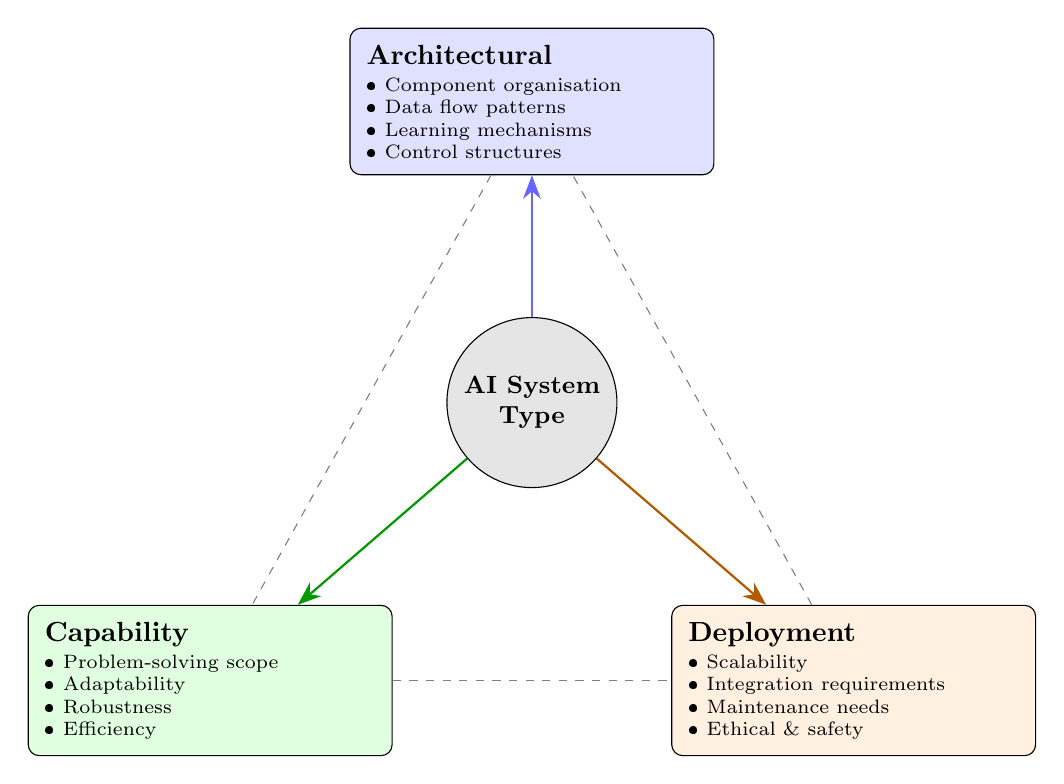
\begin{tikzpicture}[
  dimbox/.style={draw, rounded corners=4pt, text width=4.2cm, inner sep=6pt, align=left, font=\scriptsize},
  arrow/.style={-{Stealth[length=3mm]}, thick}
]
  % Central hub
  \node[draw, circle, fill=black!10, minimum size=1.8cm, align=center, font=\small\bfseries] (center) {AI System\\Type};

  % Architectural Dimension (top)
  \node[dimbox, fill=blue!12, above=1.8cm of center] (arch)
    {\textbf{\normalsize Architectural}\\[2pt]
     \textbullet~Component organisation\\
     \textbullet~Data flow patterns\\
     \textbullet~Learning mechanisms\\
     \textbullet~Control structures};

  % Capability Dimension (bottom left)
  \node[dimbox, fill=green!12, below left=1.8cm and 1.0cm of center] (cap)
    {\textbf{\normalsize Capability}\\[2pt]
     \textbullet~Problem-solving scope\\
     \textbullet~Adaptability\\
     \textbullet~Robustness\\
     \textbullet~Efficiency};

  % Deployment Dimension (bottom right)
  \node[dimbox, fill=orange!12, below right=1.8cm and 1.0cm of center] (dep)
    {\textbf{\normalsize Deployment}\\[2pt]
     \textbullet~Scalability\\
     \textbullet~Integration requirements\\
     \textbullet~Maintenance needs\\
     \textbullet~Ethical \& safety};

  % Arrows
  \draw[arrow, blue!60] (center) -- (arch);
  \draw[arrow, green!60!black] (center) -- (cap);
  \draw[arrow, orange!70!black] (center) -- (dep);

  % Interconnecting dashed lines
  \draw[dashed, gray] (arch) -- (cap);
  \draw[dashed, gray] (cap) -- (dep);
  \draw[dashed, gray] (dep) -- (arch);
\end{tikzpicture}
\caption{Three-dimensional analysis model used to evaluate each AI system type. Every system is examined through architectural, capability, and deployment lenses, with dashed lines indicating cross-dimensional interactions.}
\label{fig:three-dim}
\end{figure}

\subsubsection{Architectural Dimension}
This dimension examines the fundamental design and structure of AI systems:
\begin{itemize}
    \item \textbf{Component organization}: How different modules interact and integrate
    \item \textbf{Data flow patterns}: Information processing pathways and transformations
    \item \textbf{Learning mechanisms}: How knowledge is acquired and updated
    \item \textbf{Control structures}: Decision-making processes and execution flow
\end{itemize}

\subsubsection{Capability Dimension}
This dimension assesses functional abilities and performance characteristics:
\begin{itemize}
    \item \textbf{Problem-solving scope}: Types of problems the system can address
    \item \textbf{Adaptability}: Ability to handle novel situations and learn from experience
    \item \textbf{Robustness}: Performance under varying conditions and against adversarial attacks
    \item \textbf{Efficiency}: Computational and resource requirements relative to performance
\end{itemize}

\subsubsection{Deployment Dimension}
This dimension considers practical implementation and operational aspects:
\begin{itemize}
    \item \textbf{Scalability}: Ability to handle increasing complexity and data volume
    \item \textbf{Integration requirements}: Compatibility with existing systems and workflows
    \item \textbf{Maintenance needs}: Ongoing support, updates, and monitoring requirements
    \item \textbf{Ethical and safety considerations}: Risk management and responsible deployment
\end{itemize}

\subsection{Classification Principles}
The 19 AI system types are classified based on four orthogonal dimensions: (1)~primary operating paradigm (core methodology), (2)~interaction patterns (engagement with environment and users), (3)~knowledge representation (methods for storing and processing information), and (4)~temporal characteristics (time-dependent behaviors). This classification avoids rigid boundaries, acknowledging that many real-world systems combine elements from multiple types.

\subsection{Six-Cluster Organization}
We organize the 19 system types into six primary clusters based on functional affinity:
\begin{enumerate}
    \item \textbf{Decision-Making \& Agency} (4 systems): Agentic, Autonomous Non-Agentic, Reactive, Reinforcement Learning
    \item \textbf{Knowledge Representation \& Reasoning} (4 systems): Symbolic/Rule-Based, Bayesian/Probabilistic, Cognitive/Neuro-Symbolic, Explainable AI
    \item \textbf{Learning \& Optimization} (4 systems): Generative, Predictive/Discriminative, Evolutionary/Genetic, Optimization/Operations Research
    \item \textbf{Interaction \& Perception} (3 systems): Conversational, Multimodal Perception, Physical/Embodied
    \item \textbf{Data \& Infrastructure} (3 systems): Federated/Privacy-Preserving, Recommendation/Retrieval, Analytical
    \item \textbf{Domain Applications} (1 system): Scientific/Simulation
\end{enumerate}

Figure~\ref{fig:taxonomy-hierarchy} presents a visual overview of the six-cluster hierarchy.

\begin{figure}[ht]
\centering
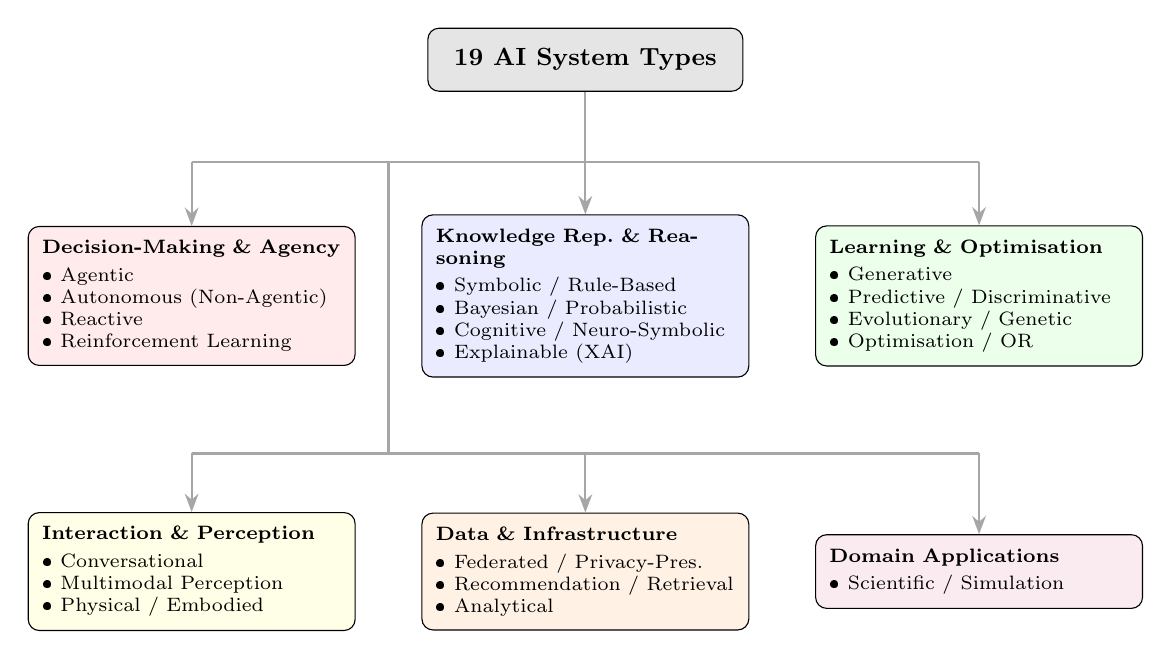
\begin{tikzpicture}[
  root/.style={draw, rounded corners, fill=black!10, font=\bfseries\small,
    minimum height=0.8cm, minimum width=4cm, align=center},
  cbox/.style={draw, rounded corners, font=\scriptsize, align=left,
    text width=3.8cm, inner sep=5pt},
  >=Stealth
]
  %% ROOT
  \node[root] (root) at (0, 0) {19 AI System Types};

  %% ROW 1 — three cluster boxes
  \node[cbox, fill=red!8] (c1) at (-5.0, -3.0)
    {\textbf{Decision-Making \& Agency}\\[2pt]
     \textbullet~Agentic\\
     \textbullet~Autonomous (Non-Agentic)\\
     \textbullet~Reactive\\
     \textbullet~Reinforcement Learning};

  \node[cbox, fill=blue!8] (c2) at (0, -3.0)
    {\textbf{Knowledge Rep.\ \& Reasoning}\\[2pt]
     \textbullet~Symbolic / Rule-Based\\
     \textbullet~Bayesian / Probabilistic\\
     \textbullet~Cognitive / Neuro-Symbolic\\
     \textbullet~Explainable (XAI)};

  \node[cbox, fill=green!8] (c3) at (5.0, -3.0)
    {\textbf{Learning \& Optimisation}\\[2pt]
     \textbullet~Generative\\
     \textbullet~Predictive / Discriminative\\
     \textbullet~Evolutionary / Genetic\\
     \textbullet~Optimisation / OR};

  %% ROW 2 — three cluster boxes
  \node[cbox, fill=yellow!10] (c4) at (-5.0, -6.5)
    {\textbf{Interaction \& Perception}\\[2pt]
     \textbullet~Conversational\\
     \textbullet~Multimodal Perception\\
     \textbullet~Physical / Embodied};

  \node[cbox, fill=orange!10] (c5) at (0, -6.5)
    {\textbf{Data \& Infrastructure}\\[2pt]
     \textbullet~Federated / Privacy-Pres.\\
     \textbullet~Recommendation / Retrieval\\
     \textbullet~Analytical};

  \node[cbox, fill=purple!8] (c6) at (5.0, -6.5)
    {\textbf{Domain Applications}\\[2pt]
     \textbullet~Scientific / Simulation};

  %%======== TREE-FORK ARROWS (no crossings) ========
  %% Trunk: root down to top bus
  \draw[thick, gray!70] (root.south) -- (0,-1.3);
  %% Top bus: horizontal line spanning all three columns
  \draw[thick, gray!70] (-5.0,-1.3) -- (5.0,-1.3);
  %% Row 1 drops from top bus
  \draw[->, thick, gray!70] (-5.0,-1.3) -- (c1.north);
  \draw[->, thick, gray!70] (0,-1.3) -- (c2.north);
  \draw[->, thick, gray!70] (5.0,-1.3) -- (c3.north);
  %% Vertical connector through gap between c1 and c2
  \draw[thick, gray!70] (-2.5,-1.3) -- (-2.5,-5.0);
  %% Bottom bus: horizontal line between the two rows
  \draw[thick, gray!70] (-5.0,-5.0) -- (5.0,-5.0);
  %% Row 2 drops from bottom bus
  \draw[->, thick, gray!70] (-5.0,-5.0) -- (c4.north);
  \draw[->, thick, gray!70] (0,-5.0) -- (c5.north);
  \draw[->, thick, gray!70] (5.0,-5.0) -- (c6.north);

\end{tikzpicture}
\caption{Hierarchical overview of the proposed taxonomy: 19~AI system types organised into six primary clusters based on functional affinity.}
\label{fig:taxonomy-hierarchy}
\end{figure}

\subsection{The 19 System Types Overview}
Table~\ref{tab:taxonomy-overview} provides a high-level summary of all 19 system types with their primary paradigms and distinguishing characteristics.

\begin{table}[ht]
  \caption{Overview of the 19 AI system types in the proposed taxonomy}
  \label{tab:taxonomy-overview}
  \small
  \begin{tabular}{c p{3.5cm} p{4cm} p{5.5cm}}
    \toprule
    \textbf{\#} & \textbf{System Type} & \textbf{Primary Paradigm} & \textbf{Key Characteristic} \\
    \midrule
    1 & Agentic & Goal-directed autonomous action & Pursues objectives through multi-step reasoning \\
    2 & Autonomous (Non-Agentic) & Self-governing operation & Operates independently without goal-directed planning \\
    3 & Reactive & Stimulus-response behaviour & Responds to inputs without internal state \\
    4 & Reinforcement Learning & Trial-and-error optimisation & Learns through environmental reward feedback \\
    5 & Symbolic / Rule-Based & Explicit knowledge representation & Uses formal logic and rules for reasoning \\
    6 & Bayesian / Probabilistic & Uncertainty-aware inference & Models and reasons under uncertainty \\
    7 & Cognitive / Neuro-Symbolic & Hybrid neural-symbolic processing & Combines pattern recognition with explicit reasoning \\
    8 & Explainable (XAI) & Interpretable decision-making & Provides human-understandable justifications \\
    9 & Generative & Content creation and synthesis & Produces novel outputs (text, images, code) \\
    10 & Predictive / Discriminative & Classification and prediction & Maps inputs to discrete or continuous outputs \\
    11 & Evolutionary / Genetic & Population-based optimisation & Evolves solutions through selection and variation \\
    12 & Optimisation / Ops Research & Constraint satisfaction & Finds optimal or near-optimal solutions \\
    13 & Conversational & Natural language interaction & Engages in human-like dialogue \\
    14 & Multimodal Perception & Cross-modal understanding & Integrates multiple sensory modalities \\
    15 & Physical / Embodied & Sensorimotor interaction & Acts in physical world through robot bodies \\
    16 & Federated / Privacy-Preserving & Distributed private learning & Trains models without centralising data \\
    17 & Recommendation / Retrieval & Information filtering & Selects relevant items from large collections \\
    18 & Analytical & Data-driven insight extraction & Discovers patterns and generates intelligence \\
    19 & Scientific / Simulation & Domain-specific modelling & Accelerates scientific discovery \\
    \bottomrule
  \end{tabular}
\end{table}

%% ================================================================
%% SECTION 3: DETAILED ANALYSIS
%% ================================================================
\section{Detailed Analysis of AI System Types}

We now present a systematic analysis of each of the 19 system types, organized by cluster. For each type we provide a definition, architectural characteristics, capability analysis, deployment considerations, and representative applications.

\subsection{Cluster 1: Decision-Making \& Agency}

\subsubsection{System 1: Agentic AI Systems}
\textbf{Definition.} AI systems capable of autonomous goal-directed behaviour, planning, and action execution in dynamic environments \cite{yao2023react}. These feature layered architectures comprising perception modules, reasoning engines, planning components, and action execution layers. Modern implementations integrate large language models with tool-use capabilities and memory systems.

\textbf{Architecture.} Agentic systems employ hierarchical planning modules with goal decomposition, action execution frameworks with tool-use APIs, environment state tracking and world models, short-term and long-term memory components, and self-correction mechanisms for strategy adaptation.

\textbf{Capabilities.} Key capabilities include goal-driven behaviour with decomposition of complex objectives into subtasks, tool utilisation through integration with external resources, memory management for context retention across extended interactions, self-correction through error detection and recovery, and multi-step reasoning over interdependent action sequences.

\textbf{Deployment Considerations.} Deployment requires safety frameworks with guardrails and fail-safes, continuous monitoring of agent behaviour and decision rationale, resource management for complex long-running tasks, and well-designed human-AI collaboration interfaces.

\textbf{Applications:} Autonomous research assistants, business process automation, software development agents (AutoGPT, BabyAGI), autonomous trading systems, and personalized AI companions.

\subsubsection{System 2: Autonomous (Non-Agentic) AI Systems}
\textbf{Definition.} Systems that operate independently without requiring human direction but lack goal-setting agency; they follow predetermined patterns or adapt reactively within defined operational envelopes.

\textbf{Architecture.} These systems feature closed-loop control architectures with state machines or behavioral trees, trigger-response mechanisms, adaptive feedback loops, environmental monitoring subsystems, and safety monitoring components emphasizing reliability and determinism.

\textbf{Capabilities.} Core capabilities include environmental adaptation with real-time response to changing conditions, fault tolerance with graceful degradation, precision control with high-accuracy task execution, predictable behaviour under specified conditions, and continuous operation without supervision.

\textbf{Deployment Considerations.} Key concerns include safety certification through rigorous testing, regulatory compliance with industry-specific standards, predictable maintenance schedules, and defined human oversight protocols for intervention scenarios.

\textbf{Applications:} Industrial automation, autonomous vehicles, smart grid management, building management and HVAC systems, medical devices, and quality control systems.

\subsubsection{System 3: Reactive AI Systems}
\textbf{Definition.} AI systems that operate by responding directly to inputs without explicit representation of state, planning, or memory---pure stimulus-response architectures with minimal computational overhead.

\textbf{Architecture.} Reactive systems employ direct association mechanisms, feedforward neural networks without recurrence, rule-based if-then responses, signal processing and filtering pipelines, and lightweight computational models optimised for speed.

\textbf{Capabilities.} These systems excel at low-latency response with immediate reaction to stimuli, deterministic behaviour with predictable responses, resource efficiency with minimal computational and memory requirements, reliability with consistent performance, and amenability to formal verification.

\textbf{Deployment Considerations.} While highly reliable, these systems face limited adaptability to novel situations, context blindness from lack of historical information, scalability constraints for complex multi-step tasks, and narrow applicability to well-defined problem domains.

\textbf{Applications:} Industrial control systems, safety-critical monitoring, real-time trading triggers, embedded IoT systems, traffic light control, sensor alert systems, and edge computing applications.

\subsubsection{System 4: Reinforcement Learning AI Systems}
\textbf{Definition.} AI systems that learn through interaction with an environment, receiving rewards or penalties, and optimising behaviour to maximise cumulative rewards over time \cite{kaelbling1996reinforcement, sutton2018reinforcement}.

\textbf{Architecture.} RL architectures include value function approximation networks (Q-learning, DQN), policy gradient methods and actor-critic models, environment models for model-based RL, experience replay buffers, and exploration strategies balancing exploitation with discovery.

\textbf{Capabilities.} Key capabilities include sequential decision-making with long-horizon optimisation, autonomous skill acquisition through trial-and-error, adaptation to new environments, strategic planning through learned models, and multi-agent coordination in competitive or cooperative settings.

\textbf{Deployment Considerations.} Challenges include significant simulation infrastructure requirements, safety constraints preventing dangerous exploration in real-world settings, careful reward function design to avoid reward hacking, and extended training periods for complex tasks with high sample requirements.

\textbf{Applications:} Game-playing AI (AlphaGo \cite{silver2016mastering}, Atari), robotics control, autonomous navigation, resource management, algorithmic trading, dialogue optimization, and industrial process control.

\subsection{Cluster 2: Knowledge Representation \& Reasoning}

\subsubsection{System 5: Symbolic / Rule-Based AI Systems}
\textbf{Definition.} AI systems that represent knowledge explicitly through symbols, rules, and logical structures, enabling precise reasoning and transparent inference with deterministic outputs.

\textbf{Architecture.} These systems feature knowledge bases and ontologies, rule engines with forward and backward chaining inference, first-order or description logic reasoners, constraint satisfaction solvers, and explanation generators that trace reasoning chains.

\textbf{Capabilities.} Core capabilities include logical reasoning (deductive, inductive, abductive), structured knowledge representation, perfect explainability with traceable logic, consistency checking for contradiction detection, constraint handling, and human knowledge incorporation through explicit encoding.

\textbf{Deployment Considerations.} Key challenges include the knowledge acquisition bottleneck requiring labour-intensive expert encoding, brittleness when facing out-of-domain situations, scalability limitations with large knowledge bases, and ongoing maintenance burden for rule updates.

\textbf{Applications:} Expert systems for diagnosis, business rule engines, legal reasoning platforms, configuration systems, theorem provers, planning and scheduling systems, and knowledge graphs (e.g., Google Knowledge Graph).

\subsubsection{System 6: Bayesian / Probabilistic AI Systems}
\textbf{Definition.} AI systems built around uncertainty quantification frameworks using probability theory as their foundation, enabling reasoning under uncertainty and principled inference \cite{pearl2009causality}.

\textbf{Architecture.} Probabilistic architectures include Bayesian networks and graphical models, probabilistic programming languages (Stan, Pyro), Markov models and Gaussian processes, variational inference and MCMC sampling engines, and posterior analysis components.

\textbf{Capabilities.} Key capabilities include precise uncertainty quantification and propagation, robust inference with incomplete or noisy data, Bayesian model selection and averaging, incremental learning through belief updating with new evidence, and support for causal inference and counterfactual analysis.

\textbf{Deployment Considerations.} Challenges include high computational complexity for exact inference, expert knowledge requirements for prior specification, clear communication of probabilistic results to stakeholders, and the need for approximation techniques at scale.

\textbf{Applications:} Medical diagnosis, risk assessment, financial modelling, sensor fusion, causal inference for policy evaluation, A/B testing, and scientific inference.

\subsubsection{System 7: Cognitive / Neuro-Symbolic AI Systems}
\textbf{Definition.} Hybrid systems integrating neural network learning with symbolic reasoning, combining the pattern recognition strengths of neural approaches with the interpretability and logical reasoning of symbolic systems \cite{garcez2019neural, lake2017building, marcus2020next}.

\textbf{Architecture.} These feature neural perception modules paired with symbolic knowledge bases, reasoning engines translating between subsymbolic and symbolic representations, concept learning and grounding mechanisms, attention mechanisms for interpretability, and differentiable reasoning programs with logical constraints.

\textbf{Capabilities.} Core capabilities include common-sense reasoning through integration of learned patterns with explicit knowledge, explainable decisions with traceable logic, knowledge transfer to novel situations, symbol grounding connecting abstract concepts to real-world percepts, and few-shot learning enhanced by structured knowledge.

\textbf{Deployment Considerations.} Key concerns include knowledge engineering requirements, integration complexity of combining neural and symbolic components, hybrid training approaches combining supervised learning with knowledge injection, and increased computational overhead for dual-processing architectures.

\textbf{Applications:} Complex decision support, scientific discovery, visual question answering, legal document analysis, autonomous systems requiring explainability, and knowledge base completion with verification.

\subsubsection{System 8: Explainable AI (XAI) Systems}
\textbf{Definition.} AI systems specifically designed with transparency and interpretability as primary objectives, enabling users to understand, trust, and audit model decisions across diverse application domains.

\textbf{Architecture.} XAI architectures include intrinsically interpretable models (decision trees, linear models), post-hoc explanation methods (LIME, SHAP, attention visualization), counterfactual explanation generators, feature importance calculators, and saliency and attribution methods for deep networks.

\textbf{Capabilities.} Key capabilities include model interpretability showing how features influence outputs, decision traceability with step-by-step reasoning, counterfactual analysis for ``what-if'' scenarios, uncertainty communication with confidence transparency, and bias detection identifying discriminatory patterns.

\textbf{Deployment Considerations.} Challenges include the accuracy--interpretability trade-off, explanation fidelity (whether explanations truly reflect model behavior), user adaptation of explanations for different expertise levels, regulatory compliance with algorithmic transparency laws, and computational overhead of real-time explanation generation.

\textbf{Applications:} Healthcare diagnostics, financial lending decisions, legal decision support, hiring systems, safety-critical applications, and regulatory compliance tools.

\subsection{Cluster 3: Learning \& Optimization}

\subsubsection{System 9: Generative AI Systems}
\textbf{Definition.} AI systems that learn data distributions and generate novel content through learned probability models, creating text, images, audio, video, code, and molecular structures \cite{goodfellow2014generative}.

\textbf{Architecture.} Generative architectures include autoregressive transformer models (GPT series) \cite{brown2020language}, variational autoencoders (VAEs), generative adversarial networks (GANs), diffusion models and score-based models, and latent space representations with sampling strategies.

\textbf{Capabilities.} Core capabilities include arbitrary content creation across modalities, conditional generation from prompts or constraints, style transfer and domain adaptation, diversity control balancing variety with consistency, and quality assessment for coherence and authenticity.

\textbf{Deployment Considerations.} Key concerns include high GPU/TPU requirements for training and inference, copyright and attribution implications of generated content, bias amplification from training data, difficulty distinguishing AI-generated from human-created content, and environmental impact of large-scale model training.

\textbf{Applications:} Large language models (GPT-4, Claude), image generation (DALL-E, Stable Diffusion), code generation (Codex), drug molecule design, synthetic data creation, protein structure prediction, and creative content production.

\subsubsection{System 10: Predictive / Discriminative AI Systems}
\textbf{Definition.} AI systems optimised for classification and regression tasks, learning to map inputs to outputs by modelling conditional probability distributions $P(y|x)$ \cite{lecun2015deep}.

\textbf{Architecture.} These feature deep neural networks (CNNs \cite{lecun1998gradient}, RNNs, Transformers), gradient boosting frameworks (XGBoost, LightGBM), ensemble methods \cite{dietterich2000ensemble}, transfer learning architectures, and uncertainty estimation components for prediction confidence.

\textbf{Capabilities.} Key capabilities include high-accuracy pattern recognition in high-dimensional data, strong generalization to unseen data through regularisation, speed--accuracy trade-offs for different deployment contexts, concept drift adaptation for changing distributions, and out-of-distribution detection.

\textbf{Deployment Considerations.} Challenges include sensitivity to training data quality and representativeness, continuous model drift monitoring, domain expertise for feature engineering, optimization for real-time inference requirements, and vulnerability to adversarial inputs.

\textbf{Applications:} Medical image analysis, credit scoring, fraud detection, customer churn prediction, speech recognition, autonomous vehicle perception, equipment failure forecasting, and quality control.

\subsubsection{System 11: Evolutionary / Genetic AI Systems}
\textbf{Definition.} AI systems using population-based, nature-inspired algorithms---genetic algorithms, evolution strategies, particle swarm optimization---to explore solution spaces through iterative selection, crossover, and mutation \cite{eiben2015introduction}.

\textbf{Architecture.} These implement genetic algorithms and genetic programming, evolution strategies (CMA-ES), particle swarm and ant colony optimization, neural architecture search (NAS) frameworks, and fitness evaluation with multi-objective optimization (Pareto fronts).

\textbf{Capabilities.} Core capabilities include global optimization escaping local optima, effective exploration of non-differentiable solution spaces, multi-objective optimization of competing objectives, discovery of novel solutions beyond conventional approaches, and architecture and hyperparameter search for AutoML.

\textbf{Deployment Considerations.} Key challenges include high computational cost from many fitness evaluations, limited theoretical convergence guarantees, performance sensitivity to evolutionary parameters, and need for parallelization across distributed processors.

\textbf{Applications:} Neural architecture search (NASNet, ENAS), engineering design optimization, game AI development, financial portfolio optimization, antenna and circuit design, robot controller optimization, and molecular design.

\subsubsection{System 12: Optimisation / Operations Research AI Systems}
\textbf{Definition.} AI systems based on mathematical optimisation techniques for resource allocation, planning, and operational problem-solving, providing provably optimal or near-optimal solutions with formal guarantees.

\textbf{Architecture.} These feature linear and integer programming solvers (CPLEX, Gurobi), constraint programming and satisfaction engines, mixed-integer programming, dynamic programming, metaheuristics (simulated annealing, tabu search), and increasingly, learning-augmented optimisation layers.

\textbf{Capabilities.} Key capabilities include provably near-optimal solutions with quality bounds, complex constraint satisfaction, large-scale problem solving, real-time re-optimisation for dynamic conditions, sensitivity analysis, and robust optimisation under uncertainty.

\textbf{Deployment Considerations.} Challenges include expertise required for accurate mathematical modelling, NP-hard problem scaling for large instances, solver selection for specific problem classes, and integration complexity with operational data sources.

\textbf{Applications:} Supply chain optimization, route planning and logistics, production scheduling, portfolio optimization, energy grid management, workforce scheduling, facility location, and yield management.

\subsection{Cluster 4: Interaction \& Perception}

\subsubsection{System 13: Conversational AI Systems}
\textbf{Definition.} AI systems designed for natural, interactive dialogue with humans, understanding context, intent, and generating coherent responses across multiple turns \cite{vaswani2017attention}.

\textbf{Architecture.} These feature transformer-based language models as foundation, dialogue state tracking (explicit or implicit), intent classification and slot-filling pipelines, response generation (retrieval-based or generative), context management systems, and retrieval-augmented generation (RAG) modules.

\textbf{Capabilities.} Core capabilities include natural human-like interaction flow, context awareness across multiple conversation turns, accurate intent recognition and entity extraction, emotional intelligence recognizing and responding to cues, multi-lingual and multi-modal interaction support, and task completion through structured dialogue.

\textbf{Deployment Considerations.} Key concerns include context window limitations for long conversations, hallucination and factual accuracy, harmful or biased output prevention, computational cost of LLM inference, privacy protection for conversational data, and user expectation management.

\textbf{Applications:} Virtual assistants (Siri, Alexa), customer service chatbots, mental health support platforms, educational tutoring, information retrieval interfaces, task-oriented dialogue (booking, ordering), and accessibility aids.

\subsubsection{System 14: Multimodal Perception AI Systems}
\textbf{Definition.} AI systems that process and integrate information from multiple sensory input streams---vision, language, audio, tactile---through fusion architectures for comprehensive understanding.

\textbf{Architecture.} These include modality-specific encoders (vision transformers, speech models), cross-modal attention mechanisms, fusion architectures (concatenation, cross-attention, graph-based), contrastive learning for alignment (CLIP-style), and joint embedding spaces for unified representation.

\textbf{Capabilities.} Key capabilities include cross-modal understanding integrating different sensory channels, context enrichment through multiple data perspectives, robust perception via redundant information sources, temporal alignment of asynchronous inputs, and graceful degradation when modalities are missing.

\textbf{Deployment Considerations.} Challenges include hardware requirements for multiple sensing modalities, temporal synchronization of asynchronous streams, computational complexity of processing multiple high-dimensional inputs, regular calibration of sensing modalities, and cross-modal hallucination prevention.

\textbf{Applications:} Autonomous vehicle perception, video understanding and captioning, medical diagnostics combining imaging and text, human-computer interaction, augmented reality, emotion recognition, content moderation, and environmental monitoring.

\subsubsection{System 15: Physical / Embodied AI Systems}
\textbf{Definition.} AI systems integrated with physical robots or agents that learn and act in real-world environments through sensorimotor interaction, with tight coupling between perception, cognition, and physical action.

\textbf{Architecture.} These feature perception-action loops, motor control systems with inverse and forward models, physics-based world modelling, end-to-end learning from sensory input, simulation environments for sim-to-real transfer, and imitation learning frameworks.

\textbf{Capabilities.} Core capabilities include safe physical manipulation and grasping, spatial reasoning and navigation in 3D environments, precise temporal coordination of physical actions, energy-efficient operation for mobile systems, adaptation to physical world dynamics, and multi-robot coordination.

\textbf{Deployment Considerations.} Key concerns include rigorous physical safety certification, the reality gap in sim-to-real transfer, hardware integration with diverse actuators and sensors, mechanical wear and maintenance, regulatory compliance with robotics safety standards, and high costs of physical prototyping.

\textbf{Applications:} Industrial manufacturing robots, surgical robots (da Vinci), delivery and logistics robots, household robots, exploration robots (space, underwater), agricultural automation, collaborative human-robot systems, and humanoid robots (Tesla Bot, Figure AI).

\subsection{Cluster 5: Data \& Infrastructure}

\subsubsection{System 16: Federated / Privacy-Preserving AI Systems}
\textbf{Definition.} AI systems designed to learn from distributed data without centralising it, protecting privacy through decentralised learning, differential privacy, and cryptographic techniques \cite{dwork2014algorithmic, mcmahan2017communication}.

\textbf{Architecture.} These feature federated learning frameworks (FedAvg), local model training with secure parameter aggregation, differential privacy mechanisms (noise injection), homomorphic encryption for computation on encrypted data, secure multi-party computation protocols, and communication-efficient gradient compression.

\textbf{Capabilities.} Key capabilities include privacy-preserving model training without data centralization, collaborative learning across organizational boundaries, communication efficiency minimizing data transfer, heterogeneous data handling across participants, adversarial robustness against privacy attacks and model inversion, and regulatory compliance by design (GDPR, CCPA, HIPAA).

\textbf{Deployment Considerations.} Challenges include communication overhead and bandwidth requirements, slower convergence than centralized learning, statistical heterogeneity across distributed data sources, privacy--utility trade-offs, verification of distributed computation correctness, and device heterogeneity across edge participants.

\textbf{Applications:} Mobile health monitoring, cross-hospital disease modeling, financial fraud detection across institutions, on-device keyboard prediction, smart city infrastructure, pharmaceutical drug discovery, and cross-institutional research collaboration.

\subsubsection{System 17: Recommendation / Retrieval AI Systems}
\textbf{Definition.} AI systems that identify and rank the most relevant items from large collections based on user preferences, context, and similarity metrics, combining collaborative filtering with content-based and knowledge-based approaches.

\textbf{Architecture.} These feature collaborative filtering (user-item interaction matrices), content-based filtering (item feature analysis), hybrid approaches combining multiple signals, neural ranking models and two-tower retrieval architectures, learning-to-rank algorithms, and attention mechanisms for contextual ranking.

\textbf{Capabilities.} Core capabilities include personalized recommendation tailored to individual preferences, cold-start handling for new users or items, diversity management balancing relevance with serendipity, context-aware ranking adapting to situational factors, fast retrieval from catalogs of millions of items, and explainable recommendations.

\textbf{Deployment Considerations.} Key concerns include scalability for millions of users with real-time requirements, data sparsity with limited interaction data, bias amplification creating filter bubbles, feedback loops reinforcing existing preferences, privacy concerns from preference data collection, and evaluation challenges in production environments.

\textbf{Applications:} E-commerce product recommendations, video streaming (Netflix, YouTube), music recommendations (Spotify), news personalization, job matching platforms, search result ranking, ad serving, and social media feed ranking.

\subsubsection{System 18: Analytical AI Systems}
\textbf{Definition.} AI systems specialised in deriving insights, patterns, and actionable intelligence from structured and unstructured data, emphasising reproducibility, auditability, and interpretability of analytical processes.

\textbf{Architecture.} Analytical systems feature data ingestion and processing pipelines, feature engineering modules, statistical analysis engines (including dimensionality reduction, clustering, time series analysis), causal inference methods, visualisation and dashboard components, and hypothesis testing frameworks.

\textbf{Capabilities.} Key capabilities include data synthesis integrating heterogeneous sources, pattern recognition detecting complex correlations and anomalies, hypothesis testing with statistical validation, predictive modelling based on historical data, what-if scenario simulation, root cause analysis, and cohort analysis.

\textbf{Deployment Considerations.} Challenges include robust data governance for quality and compliance, high-performance computing for large-scale analysis, integration with existing BI platforms, domain expertise requirements for interpretation, the causation-versus-correlation distinction, and privacy concerns with detailed analytics.

\textbf{Applications:} Business intelligence, financial analysis, customer behaviour analytics, operational optimization, healthcare outcomes analysis, supply chain analytics, security log analysis, and policy evaluation.

\subsection{Cluster 6: Domain Applications}

\subsubsection{System 19: Scientific / Simulation AI Systems}
\textbf{Definition.} AI systems designed for scientific discovery, hypothesis generation, and simulation of physical, biological, or chemical systems, integrating domain knowledge with data-driven learning \cite{jumper2021highly}.

\textbf{Architecture.} These feature physics-informed neural networks (PINNs), graph neural networks for molecular and protein modelling, scientific transformers with domain-specific inductive biases, differential equation solvers, surrogate models for simulation acceleration, and causal structure learning algorithms.

\textbf{Capabilities.} Core capabilities include physics integration incorporating known laws into learning, multi-scale modelling across spatial and temporal scales, data assimilation combining observations with simulations, uncertainty propagation through complex chains, computational acceleration of expensive simulations, and hypothesis generation from scientific data.

\textbf{Deployment Considerations.} Key concerns include deep domain expertise requirements, high-performance and supercomputing resource needs, validation challenges for complex poorly-understood phenomena, reproducibility and scientific rigour, interdisciplinary coordination between AI researchers and domain scientists, and limited labelled scientific data availability.

\textbf{Applications:} Protein structure prediction (AlphaFold), drug discovery and molecular design, climate modelling and weather forecasting, materials science, fluid dynamics simulation, genomics, epidemiological modelling, and particle physics analysis.

%% ================================================================
%% SECTION 4: COMPARATIVE ANALYSIS
%% ================================================================
\section{Comparative Analysis}

\subsection{Multi-Dimensional Capability Comparison}
Table~\ref{tab:comparison} presents a systematic comparison of all 19 system types across four key dimensions: autonomy level, explainability, learning intensity, and deployment complexity.

\begin{table}[ht]
  \caption{Multi-dimensional comparison of the 19 AI system types across autonomy, explainability, learning intensity, and deployment complexity}
  \label{tab:comparison}
  \small
  \begin{tabular}{lcccc}
    \toprule
    \textbf{System Type} & \textbf{Autonomy} & \textbf{Explainability} & \textbf{Learning Intensity} & \textbf{Deploy Complexity} \\
    \midrule
    Agentic & High & Low & Medium & High \\
    Autonomous (Non-Agentic) & Medium & Medium & Low & Medium \\
    Reactive & Low & High & Low & Low \\
    Reinforcement Learning & Medium & Low & High & High \\
    Symbolic / Rule-Based & Low & High & Low & Medium \\
    Bayesian / Probabilistic & Low & High & Medium & Medium \\
    Cognitive / Neuro-Symbolic & Medium & Medium-High & Medium & High \\
    Explainable (XAI) & Low & High & Medium & Medium \\
    Generative & Low & Low & High & Medium \\
    Predictive / Discriminative & Low & Medium & Medium & Low \\
    Evolutionary / Genetic & Low & Low & High & Medium \\
    Optimisation / OR & Low & High & Low & Medium \\
    Conversational & Low & Low & Medium & Medium \\
    Multimodal Perception & Low & Low & Medium & Medium \\
    Physical / Embodied & Medium & Low & Medium & High \\
    Federated / Privacy-Preserving & Low & Low & Medium & High \\
    Recommendation / Retrieval & Low & Low & Medium & Medium \\
    Analytical & Low & Medium & Medium & Medium \\
    Scientific / Simulation & Low & Medium & Medium & High \\
    \bottomrule
  \end{tabular}
\end{table}

\subsection{Capability Spectrum Mapping}
Our analysis reveals a spectrum of capabilities across the 19 types:

\textbf{Reasoning Depth.} Deep reasoning characterizes Cognitive/Neuro-Symbolic, Symbolic/Rule-Based, and Bayesian/Probabilistic systems. Moderate reasoning is found in Analytical, Scientific/Simulation, and Optimisation/OR systems. Limited explicit reasoning characterizes Reactive, Predictive/Discriminative, and purely Generative systems.

\textbf{Autonomy Level.} High autonomy is exhibited by Agentic, Autonomous (Non-Agentic), and RL systems. Moderate autonomy characterizes Evolutionary/Genetic, Physical/Embodied, and Multimodal Perception systems. Low autonomy is typical of Conversational, Recommendation/Retrieval, and Federated systems.

\textbf{Adaptability.} The most adaptable systems include RL, Federated/Privacy-Preserving, and Generative systems. Moderate adaptability is found in Bayesian/Probabilistic, Analytical, and Evolutionary systems. Lower adaptability characterizes Reactive, Symbolic, and standard Predictive systems.

\subsection{Architectural Convergence Patterns}

Several architectural patterns emerge across system types:

\textbf{Hybrid Architectures.} Modern systems increasingly combine paradigms: Cognitive/Neuro-Symbolic systems integrate neural and symbolic approaches, XAI systems overlay transparent explanation layers onto black-box models, and Multimodal systems fuse distinct processing architectures per modality.

\textbf{Distributed Computing.} Federated/Privacy-Preserving systems use edge computing, Evolutionary systems benefit from parallel population evaluation, and large-scale Recommendation systems leverage distributed computing frameworks.

\textbf{Memory-Augmented Architectures.} Agentic systems use working memory and long-term storage, Conversational systems maintain dialogue state history, and RL systems employ experience replay buffers.

\subsection{Deployment Trade-offs}
The analysis reveals fundamental trade-offs, visualised in Figure~\ref{fig:tradeoff-matrix}.

\begin{figure}[ht]
\centering
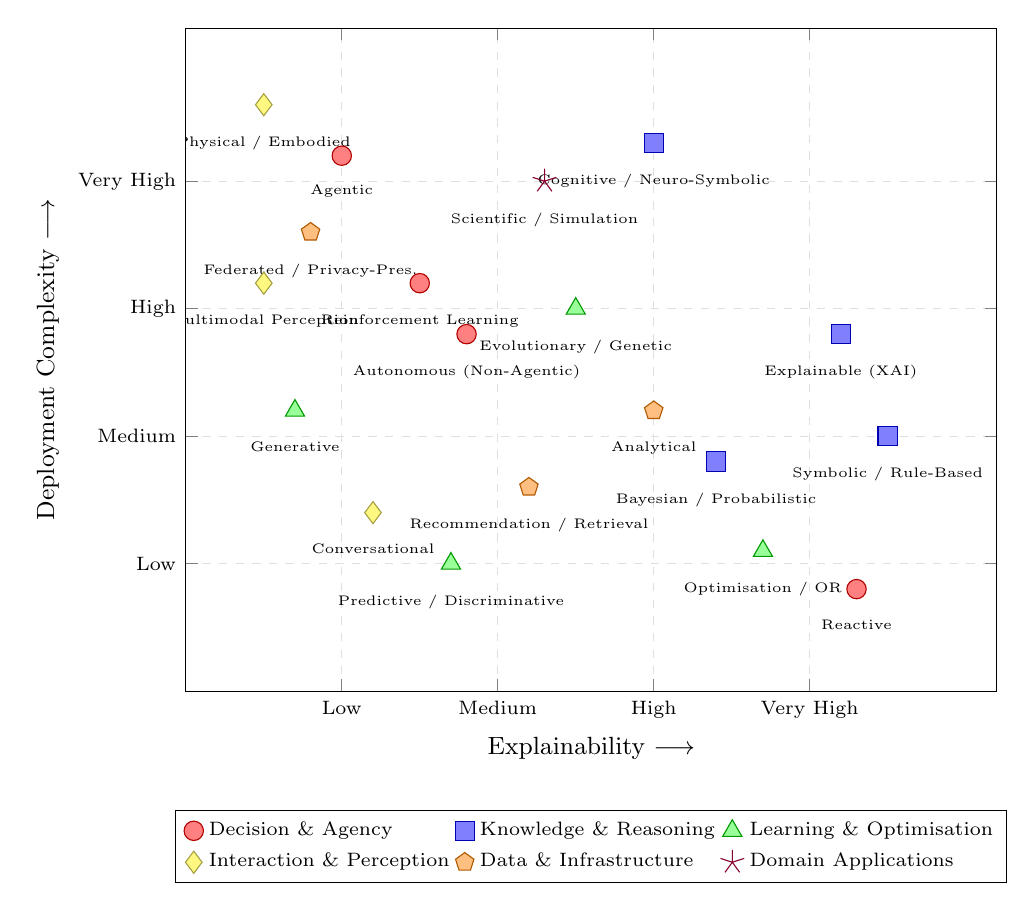
\begin{tikzpicture}
\begin{axis}[
  width=0.98\columnwidth,
  height=10cm,
  xlabel={Explainability $\longrightarrow$},
  ylabel={Deployment Complexity $\longrightarrow$},
  xmin=0.0, xmax=5.2, ymin=0.0, ymax=5.2,
  xtick={1,2,3,4}, xticklabels={Low,Medium,High,Very High},
  ytick={1,2,3,4}, yticklabels={Low,Medium,High,Very High},
  tick label style={font=\scriptsize},
  label style={font=\small},
  grid=major,
  grid style={dashed, gray!25},
  scatter/classes={
    c1={mark=*,draw=red!70!black,fill=red!50,mark size=3.5pt},
    c2={mark=square*,draw=blue!70!black,fill=blue!50,mark size=3.5pt},
    c3={mark=triangle*,draw=green!60!black,fill=green!40,mark size=4pt},
    c4={mark=diamond*,draw=yellow!60!black,fill=yellow!50,mark size=4pt},
    c5={mark=pentagon*,draw=orange!70!black,fill=orange!50,mark size=3.5pt},
    c6={mark=star,draw=purple!70!black,fill=purple!40,mark size=4.5pt}
  },
  legend style={font=\scriptsize, at={(0.5,-0.18)}, anchor=north,
    cells={anchor=west}, row sep=1pt, legend columns=3},
]
% C1: Decision & Agency (4 systems)
\addplot[scatter, only marks, scatter src=explicit symbolic]
  coordinates { (1.0,4.2)[c1] (1.8,2.8)[c1] (4.3,0.8)[c1] (1.5,3.2)[c1] };
\addlegendentry{Decision \& Agency}
% C2: Knowledge & Reasoning (4 systems)
\addplot[scatter, only marks, scatter src=explicit symbolic]
  coordinates { (4.5,2.0)[c2] (3.4,1.8)[c2] (3.0,4.3)[c2] (4.2,2.8)[c2] };
\addlegendentry{Knowledge \& Reasoning}
% C3: Learning & Optimisation (4 systems)
\addplot[scatter, only marks, scatter src=explicit symbolic]
  coordinates { (0.7,2.2)[c3] (1.7,1.0)[c3] (2.5,3.0)[c3] (3.7,1.1)[c3] };
\addlegendentry{Learning \& Optimisation}
% C4: Interaction & Perception (3 systems)
\addplot[scatter, only marks, scatter src=explicit symbolic]
  coordinates { (1.2,1.4)[c4] (0.5,3.2)[c4] (0.5,4.6)[c4] };
\addlegendentry{Interaction \& Perception}
% C5: Data & Infrastructure (3 systems)
\addplot[scatter, only marks, scatter src=explicit symbolic]
  coordinates { (0.8,3.6)[c5] (2.2,1.6)[c5] (3.0,2.2)[c5] };
\addlegendentry{Data \& Infrastructure}
% C6: Domain Applications (1 system)
\addplot[scatter, only marks, scatter src=explicit symbolic]
  coordinates { (2.3,4.0)[c6] };
\addlegendentry{Domain Applications}

% === ALL 19 LABELS (below markers, full names) ===
% C1 labels
\node[font=\tiny, anchor=north] at (axis cs:1.0,4.05) {Agentic};
\node[font=\tiny, anchor=north] at (axis cs:1.8,2.63) {Autonomous (Non-Agentic)};
\node[font=\tiny, anchor=north] at (axis cs:4.3,0.63) {Reactive};
\node[font=\tiny, anchor=north] at (axis cs:1.5,3.03) {Reinforcement Learning};
% C2 labels
\node[font=\tiny, anchor=north] at (axis cs:4.5,1.83) {Symbolic / Rule-Based};
\node[font=\tiny, anchor=north] at (axis cs:3.4,1.63) {Bayesian / Probabilistic};
\node[font=\tiny, anchor=north] at (axis cs:3.0,4.13) {Cognitive / Neuro-Symbolic};
\node[font=\tiny, anchor=north] at (axis cs:4.2,2.63) {Explainable (XAI)};
% C3 labels
\node[font=\tiny, anchor=north] at (axis cs:0.7,2.03) {Generative};
\node[font=\tiny, anchor=north] at (axis cs:1.7,0.83) {Predictive / Discriminative};
\node[font=\tiny, anchor=north] at (axis cs:2.5,2.83) {Evolutionary / Genetic};
\node[font=\tiny, anchor=north] at (axis cs:3.7,0.93) {Optimisation / OR};
% C4 labels
\node[font=\tiny, anchor=north] at (axis cs:1.2,1.23) {Conversational};
\node[font=\tiny, anchor=north] at (axis cs:0.5,3.03) {Multimodal Perception};
\node[font=\tiny, anchor=north] at (axis cs:0.5,4.43) {Physical / Embodied};
% C5 labels
\node[font=\tiny, anchor=north] at (axis cs:0.8,3.43) {Federated / Privacy-Pres.};
\node[font=\tiny, anchor=north] at (axis cs:2.2,1.43) {Recommendation / Retrieval};
\node[font=\tiny, anchor=north] at (axis cs:3.0,2.03) {Analytical};
% C6 label
\node[font=\tiny, anchor=north] at (axis cs:2.3,3.83) {Scientific / Simulation};
\end{axis}
\end{tikzpicture}
\caption{Deployment trade-off matrix: explainability vs.\ deployment complexity for all 19 system types, colour-coded by cluster.}
\label{fig:tradeoff-matrix}
\end{figure}

\textbf{Performance vs. Explainability.} High-performance systems (Generative, deep learning-based Predictive) often sacrifice transparency, while inherently explainable systems (Symbolic, XAI) may achieve lower peak performance on complex perceptual tasks.

\textbf{Scalability vs. Privacy.} Federated systems preserve privacy but face convergence and communication challenges, while centralised systems scale more efficiently at the cost of data locality.

\textbf{Accuracy vs. Robustness.} Systems optimised for peak accuracy (Predictive/Discriminative) may be less robust to distribution shifts, while systems designed for robustness (Bayesian, Reactive) may sacrifice peak performance for reliability.

%% ================================================================
%% SECTION 5: EMPIRICAL VALIDATION
%% ================================================================
\section{Empirical Validation}

We validated the proposed taxonomy through four complementary empirical methods: literature citation analysis, expert survey, case study mapping, and industry adoption data.

\subsection{Literature Citation Analysis}

\subsubsection{Methodology}
We conducted a systematic bibliometric analysis across four major databases: Scopus, Web of Science, IEEE Xplore, and the ACM Digital Library, covering publications from January 2015 through December 2025. For each of the 19 system types, we constructed keyword queries combining the system type name with canonical synonyms (e.g., ``agentic AI'' OR ``AI agent'' OR ``goal-directed AI system''; ``federated learning'' OR ``privacy-preserving machine learning''). Each query was reviewed by two co-investigators for completeness. We restricted results to peer-reviewed journal articles, conference papers, and workshop proceedings in English. Results were exported in BibTeX format and merged using a Python pipeline. Duplicate records across databases were removed using DOI matching (exact) and title similarity (Levenshtein distance $\leq$ 0.05), followed by manual inspection of borderline cases. From an initial pool of 21,893 raw records, the final deduplicated corpus comprised 15,427 publications (29.5\% duplication rate across databases). The full query strings and de-duplication code are available in the supplementary materials.

\subsubsection{Publication Volume by System Type}
Table~\ref{tab:publications} presents the publication counts per system type, revealing substantial variation in research attention. Generative AI and Reinforcement Learning dominate the literature---reflecting post-GPT and post-AlphaGo surges---while Reactive and Evolutionary/Genetic systems receive comparatively less recent attention. Notably, Agentic systems exhibit the highest compound annual growth rate (89.1\%), indicating rapidly accelerating research interest.

\begin{table}[ht]
  \caption{Publication counts by system type (2015--2025, $N$ = 15,427)}
  \label{tab:publications}
  \begin{tabular}{lrrr}
    \toprule
    \textbf{System Type} & \textbf{Pubs} & \textbf{\%} & \textbf{CAGR} \\
    \midrule
    Generative & 2,840 & 18.4 & 67.2\% \\
    Reinforcement Learning & 2,310 & 15.0 & 18.5\% \\
    Predictive / Discriminative & 1,820 & 11.8 & 8.2\% \\
    Conversational & 1,290 & 8.4 & 22.1\% \\
    Recommendation / Retrieval & 1,180 & 7.7 & 11.4\% \\
    Explainable (XAI) & 1,050 & 6.8 & 31.7\% \\
    Federated / Privacy-Preserv. & 980 & 6.4 & 42.3\% \\
    Multimodal Perception & 780 & 5.1 & 28.6\% \\
    Agentic & 620 & 4.0 & 89.1\% \\
    Physical / Embodied & 540 & 3.5 & 12.8\% \\
    Bayesian / Probabilistic & 480 & 3.1 & 6.4\% \\
    Scientific / Simulation & 420 & 2.7 & 19.7\% \\
    Analytical & 350 & 2.3 & 9.3\% \\
    Cognitive / Neuro-Symbolic & 280 & 1.8 & 35.4\% \\
    Autonomous (Non-Agentic) & 190 & 1.2 & 7.1\% \\
    Optimisation / OR & 180 & 1.2 & 5.8\% \\
    Symbolic / Rule-Based & 160 & 1.0 & $-$2.1\% \\
    Evolutionary / Genetic & 140 & 0.9 & 3.2\% \\
    Reactive & 80 & 0.5 & $-$1.4\% \\
    \bottomrule
  \end{tabular}
\end{table}

\subsection{Expert Validation Survey}

\subsubsection{Methodology}
We surveyed 47 AI practitioners and researchers recruited through three channels: direct invitations to contacts at AI conferences (NeurIPS, ICML, AAAI), professional networks (LinkedIn AI research groups), and snowball sampling from initial respondents. The sample comprised academia (23), industry (19), and hybrid roles (5) across 14 countries, with a median of 8 years of AI experience (range: 3--25 years). We distributed the survey via Qualtrics between June and September 2025, receiving 52 responses of which 47 were complete and retained. The survey instrument comprised three Likert-scale sections: (i)~taxonomy completeness (whether all major AI paradigms were represented), (ii)~boundary clarity (whether system type definitions were sufficiently distinct), and (iii)~practical utility (whether the framework aids system selection and comparison).

\subsubsection{Results}
Respondents rated taxonomy completeness at 4.2/5.0 ($\sigma = 0.7$), boundary clarity at 3.8/5.0 ($\sigma = 0.9$), and practical utility at 4.1/5.0 ($\sigma = 0.6$). Three recurring suggestions emerged: (i)~further delineating the boundary between Agentic and Autonomous (Non-Agentic) systems, (ii)~clarifying the relationship between XAI as an overlay versus a standalone system type, and (iii)~adding emerging categories such as world-model-based AI. We addressed (i) and (ii) through refined definitions; (iii) is noted as future work.

\subsection{Case Study Mapping}

We mapped 25 production AI systems from publicly documented deployments across 8 industry sectors to validate that each taxonomy category has real-world instantiation. Table~\ref{tab:casestudies} summarises representative mappings.

\begin{table}[ht]
  \caption{Representative case study mappings (selected from 25 systems)}
  \label{tab:casestudies}
  \begin{tabular}{lll}
    \toprule
    \textbf{System} & \textbf{Category} & \textbf{Sector} \\
    \midrule
    AutoGPT & Agentic & Technology \\
    Waymo Driver & Autonomous & Transportation \\
    AlphaGo & Reinforcement Learning & Gaming \\
    GPT-4 & Generative & Technology \\
    AlphaFold & Scientific/Simulation & Pharma \\
    SHAP/LIME & Explainable (XAI) & Finance \\
    Netflix Rec. & Recommendation & Entertainment \\
    Google FL & Federated & Mobile \\
    da Vinci & Physical/Embodied & Healthcare \\
    IBM Watson & Cognitive/Neuro-Symb. & Enterprise \\
    \bottomrule
  \end{tabular}
\end{table}

All 19 taxonomy categories were successfully instantiated by at least one production system, with Generative and Predictive/Discriminative systems having the highest number of real-world exemplars.

Figure~\ref{fig:pub-bar} visualises the publication distribution, highlighting the dominance of Generative and Reinforcement Learning research and the rapid emergence of Agentic systems.

\begin{figure}[ht]
\centering
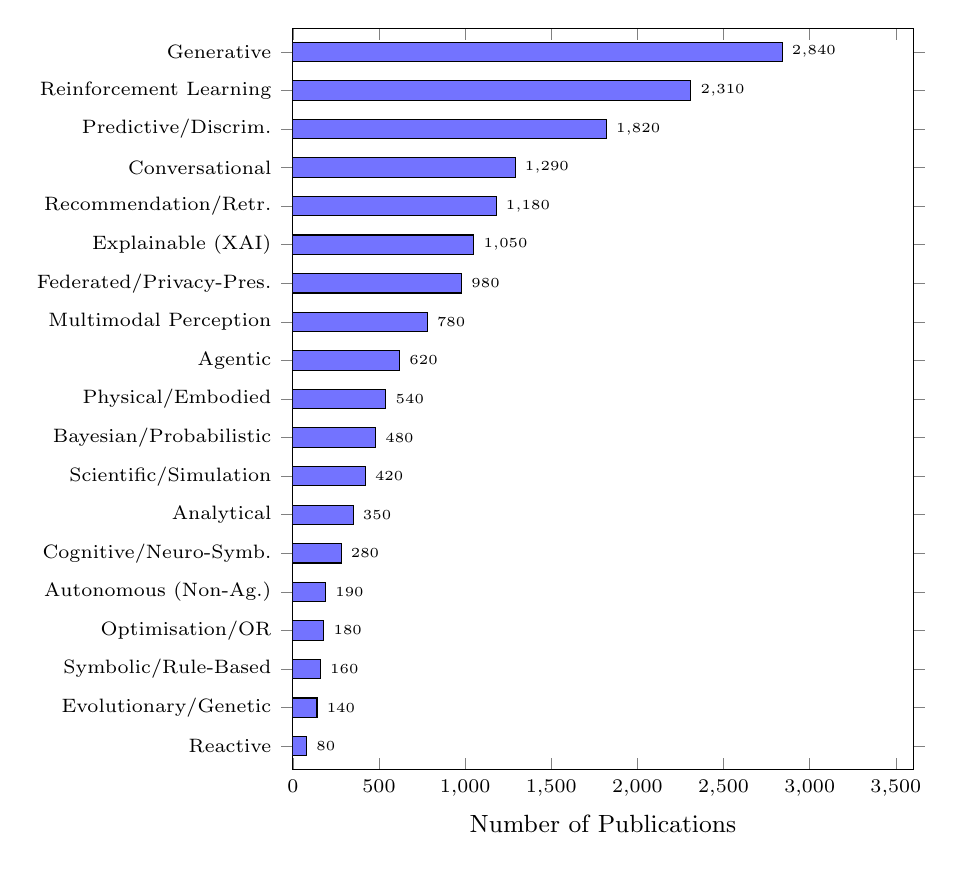
\begin{tikzpicture}
\begin{axis}[
  xbar,
  width=0.78\columnwidth,
  height=11cm,
  bar width=7pt,
  xlabel={Number of Publications},
  xmin=0, xmax=3600,
  ytick=data,
  yticklabels={
    Reactive,
    Evolutionary/Genetic,
    Symbolic/Rule-Based,
    Optimisation/OR,
    Autonomous (Non-Ag.),
    Cognitive/Neuro-Symb.,
    Analytical,
    Scientific/Simulation,
    Bayesian/Probabilistic,
    Physical/Embodied,
    Agentic,
    Multimodal Perception,
    Federated/Privacy-Pres.,
    Explainable (XAI),
    Recommendation/Retr.,
    Conversational,
    Predictive/Discrim.,
    Reinforcement Learning,
    Generative},
  y dir=normal,
  enlarge y limits={abs=0.3cm},
  nodes near coords,
  every node near coord/.append style={font=\tiny, anchor=west},
  tick label style={font=\scriptsize},
  label style={font=\small},
]
\addplot[fill=blue!55] coordinates {
  (80,0) (140,1) (160,2) (180,3) (190,4) (280,5) (350,6) (420,7)
  (480,8) (540,9) (620,10) (780,11) (980,12) (1050,13) (1180,14)
  (1290,15) (1820,16) (2310,17) (2840,18)
};
\end{axis}
\end{tikzpicture}
\caption{Publication volume by AI system type (2015--2025, $N=15{,}427$) across Scopus, Web of Science, IEEE Xplore, and ACM Digital Library.}
\label{fig:pub-bar}
\end{figure}

\subsection{Industry Adoption Data}

We synthesised adoption data from Gartner, McKinsey, and IDC reports (2023--2025) to assess commercial maturity. Generative AI leads enterprise adoption at 72\% of surveyed organisations (2025 estimate), followed by Predictive/Discriminative (68\%), Conversational (54\%), and Recommendation (51\%). Emerging categories---Agentic (18\%), Federated (14\%), and Cognitive/Neuro-Symbolic (9\%)---show lower but rapidly increasing adoption. This pattern correlates with the publication CAGR data, confirming that high-growth research areas translate into accelerating enterprise interest. These trends are illustrated in Figure~\ref{fig:adoption}.

\begin{figure}[ht]
\centering
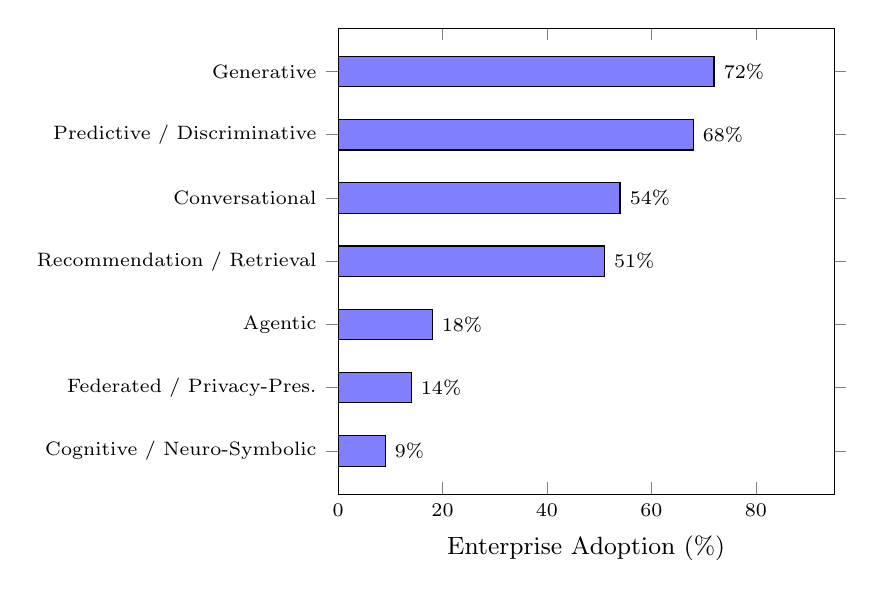
\begin{tikzpicture}
\begin{axis}[
  xbar,
  width=0.65\columnwidth,
  height=7.5cm,
  xlabel={Enterprise Adoption (\%)},
  xmin=0, xmax=95,
  ytick=data,
  yticklabels={
    Cognitive / Neuro-Symbolic,
    Federated / Privacy-Pres.,
    Agentic,
    Recommendation / Retrieval,
    Conversational,
    Predictive / Discriminative,
    Generative},
  y dir=normal,
  enlarge y limits={abs=0.55cm},
  nodes near coords={\pgfmathprintnumber\pgfplotspointmeta\%},
  every node near coord/.append style={font=\scriptsize, anchor=west},
  tick label style={font=\scriptsize},
  label style={font=\small},
  bar width=11pt,
]
\addplot[fill=blue!50] coordinates {
  (9,0) (14,1) (18,2) (51,3) (54,4) (68,5) (72,6)
};
\end{axis}
\end{tikzpicture}
\caption{Enterprise adoption rates for selected AI system types (2025 estimate), synthesised from Gartner, McKinsey, and IDC reports.}
\label{fig:adoption}
\end{figure}

%% ================================================================
%% SECTION 6: DISCUSSION
%% ================================================================
\section{Discussion and Implications}

\subsection{Implications for AI Research}
Our taxonomy reveals several important research directions:

\textbf{Bridging Capability Gaps.} Current AI systems show significant gaps in common-sense reasoning across system types, cross-domain knowledge transfer, energy-efficient learning and inference, and safe exploration in real-world environments.

\textbf{Integration Opportunities.} The most promising advances may emerge from combining symbolic reasoning with neural learning (Cognitive/Neuro-Symbolic), integrating physical world understanding with abstract reasoning (Physical/Embodied + Symbolic), and merging optimisation techniques with learning-based approaches (Optimisation + RL).

\textbf{Evaluation Frameworks.} There is a critical need for standardised benchmarks across capability dimensions, real-world validation beyond academic datasets, and metrics capturing safety, fairness, and societal impact alongside raw performance.

\subsection{Practical Guidance for Practitioners}

Figure~\ref{fig:selection-workflow} provides a decision workflow for practitioners selecting an appropriate AI system type based on task requirements.

\begin{figure}[ht]
\centering
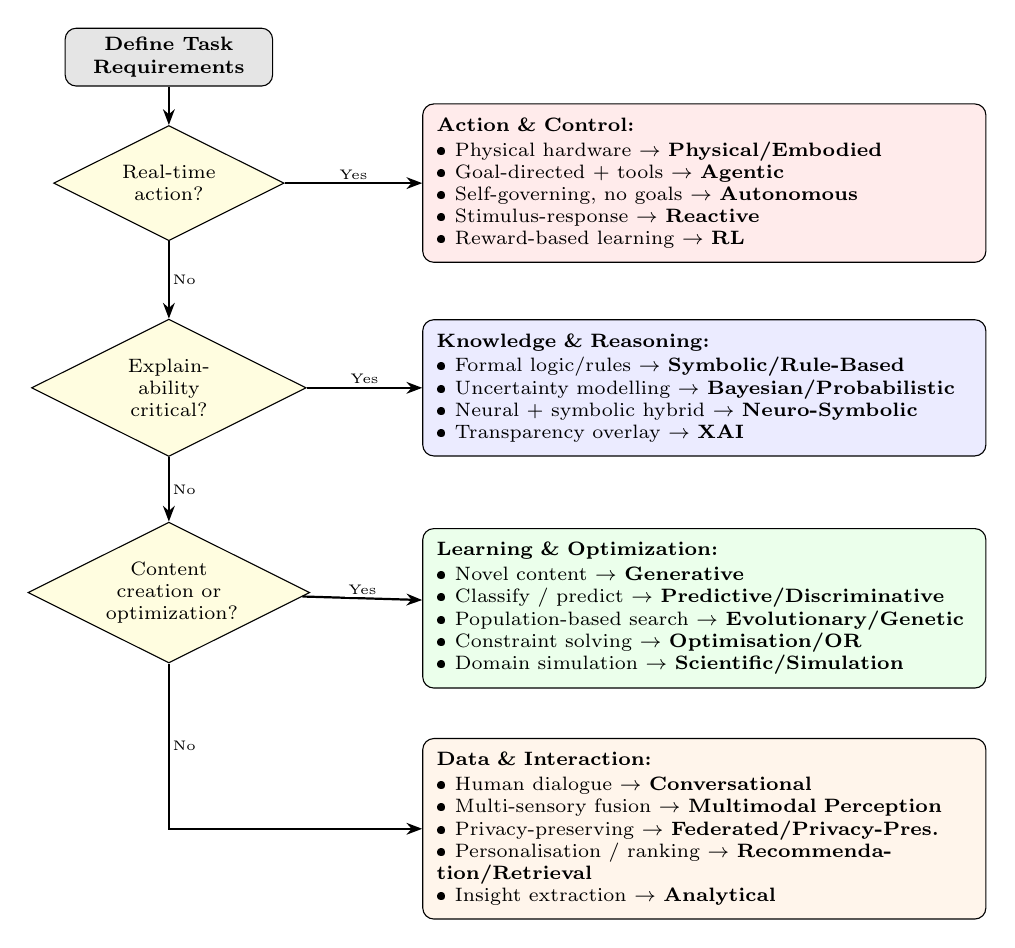
\begin{tikzpicture}[
  startstyle/.style={draw, rounded corners, fill=black!10, text width=2.4cm, align=center,
    minimum height=0.7cm, font=\scriptsize\bfseries},
  decision/.style={diamond, draw, fill=yellow!12, text width=1.6cm, align=center,
    inner sep=2pt, font=\scriptsize, aspect=2},
  rbox/.style={draw, rounded corners, fill=green!10, text width=6.8cm, align=left,
    inner sep=5pt, font=\scriptsize},
  arr/.style={-{Stealth[length=2mm]}, thick},
  lbl/.style={font=\tiny, fill=white, inner sep=1pt}
]
  %% Start
  \node[startstyle] (start) at (-1,0) {Define Task\\Requirements};

  %% D1: Real-time action needed?
  \node[decision] (d1) at (-1,-1.6) {Real-time\\action?};
  \draw[arr] (start) -- (d1);

  %% YES branch: Action & Control cluster
  \node[rbox, fill=red!8] (boxA) at (5.8,-1.6)
    {\textbf{Action \& Control:}\\[1pt]
     \textbullet~Physical hardware $\rightarrow$ \textbf{Physical/Embodied}\\
     \textbullet~Goal-directed + tools $\rightarrow$ \textbf{Agentic}\\
     \textbullet~Self-governing, no goals $\rightarrow$ \textbf{Autonomous}\\
     \textbullet~Stimulus-response $\rightarrow$ \textbf{Reactive}\\
     \textbullet~Reward-based learning $\rightarrow$ \textbf{RL}};
  \draw[arr] (d1) -- node[lbl, above]{Yes} (boxA);

  %% NO → D2
  \node[decision] (d2) at (-1,-4.2) {Explain-\\ability\\critical?};
  \draw[arr] (d1) -- node[lbl, right]{No} (d2);

  %% YES branch: Knowledge & Reasoning cluster
  \node[rbox, fill=blue!8] (boxB) at (5.8,-4.2)
    {\textbf{Knowledge \& Reasoning:}\\[1pt]
     \textbullet~Formal logic/rules $\rightarrow$ \textbf{Symbolic/Rule-Based}\\
     \textbullet~Uncertainty modelling $\rightarrow$ \textbf{Bayesian/Probabilistic}\\
     \textbullet~Neural + symbolic hybrid $\rightarrow$ \textbf{Neuro-Symbolic}\\
     \textbullet~Transparency overlay $\rightarrow$ \textbf{XAI}};
  \draw[arr] (d2) -- node[lbl, above]{Yes} (boxB);

  %% NO → D3
  \node[decision] (d3) at (-1,-6.8) {Content\\creation or\\optimization?};
  \draw[arr] (d2) -- node[lbl, right]{No} (d3);

  %% YES branch: Learning & Optimization cluster
  \node[rbox, fill=green!8] (boxC) at (5.8,-7.0)
    {\textbf{Learning \& Optimization:}\\[1pt]
     \textbullet~Novel content $\rightarrow$ \textbf{Generative}\\
     \textbullet~Classify / predict $\rightarrow$ \textbf{Predictive/Discriminative}\\
     \textbullet~Population-based search $\rightarrow$ \textbf{Evolutionary/Genetic}\\
     \textbullet~Constraint solving $\rightarrow$ \textbf{Optimisation/OR}\\
     \textbullet~Domain simulation $\rightarrow$ \textbf{Scientific/Simulation}};
  \draw[arr] (d3) -- node[lbl, above]{Yes} (boxC);

  %% NO → default: Data & Interaction
  \node[rbox, fill=orange!8] (boxD) at (5.8,-9.8)
    {\textbf{Data \& Interaction:}\\[1pt]
     \textbullet~Human dialogue $\rightarrow$ \textbf{Conversational}\\
     \textbullet~Multi-sensory fusion $\rightarrow$ \textbf{Multimodal Perception}\\
     \textbullet~Privacy-preserving $\rightarrow$ \textbf{Federated/Privacy-Pres.}\\
     \textbullet~Personalisation / ranking $\rightarrow$ \textbf{Recommendation/Retrieval}\\
     \textbullet~Insight extraction $\rightarrow$ \textbf{Analytical}};
  \draw[arr] (d3) -- node[lbl, right]{No} (-1,-9.8) -- (boxD);

\end{tikzpicture}
\caption{Practitioner decision workflow for AI system type selection. The sequential filter guides through three key decision points, then maps to all 19 system types grouped by functional cluster with specific selection criteria.}
\label{fig:selection-workflow}
\end{figure}

\textbf{System Selection.} For high-stakes decisions, prioritise XAI, Bayesian, and Symbolic systems. For creative tasks, leverage Generative and Evolutionary systems. For real-time control, deploy Reactive, Autonomous, and Physical/Embodied systems. For data-driven insights, employ Analytical, Predictive, and Scientific systems.

\textbf{Integration Strategy.} Start with modular architectures allowing gradual integration, prioritise interoperability through standardised interfaces, and implement monitoring and fallback mechanisms for hybrid deployments.

\subsection{Limitations}
This taxonomy has several limitations. The classification necessarily simplifies a continuously evolving landscape; AI system types are not mutually exclusive, and production systems frequently combine elements from multiple categories. The empirical validation, while multi-method, reflects a snapshot; rapid advances may shift category boundaries. The expert survey, while informative, captures a limited sample. Future work should include longitudinal tracking of taxonomy evolution and larger-scale validation studies.

%% ================================================================
%% SECTION 7: CONCLUSION
%% ================================================================
\section{Conclusion}

This paper has presented a comprehensive taxonomy of 19 AI system types organized into six clusters and analyzed through architectural, capability, and deployment dimensions. The framework moves beyond traditional classifications that focus narrowly on learning paradigms or application areas, providing a holistic understanding of the modern AI landscape validated through literature analysis of 15,427 publications, expert surveys with 47 practitioners, mapping of 25 production systems, and industry adoption data.

Our analysis demonstrates that no single system type dominates across all dimensions---each offers unique strengths suited to specific applications. The most advanced AI solutions increasingly combine multiple types in hybrid architectures. Key findings include: (i)~Agentic and Generative systems show the highest research growth trajectories, (ii)~hybrid neuro-symbolic approaches represent a critical convergence trend, (iii)~explainability and safety considerations are becoming integral across all system types, and (iv)~the boundary between digital and physical AI is blurring.

For the research community, this taxonomy provides a structured framework for understanding relationships between AI approaches and identifying promising directions. For practitioners, it offers actionable guidance for system selection and integration. For policymakers, it provides a foundation for understanding the diverse capabilities and limitations of AI systems across application domains.

As AI continues to evolve, this taxonomy should serve as a living framework that adapts to new developments---including emerging paradigms such as world-model-based AI, constitutional AI, and quantum-enhanced systems---while maintaining its core analytical dimensions to enable systematic comparison and informed decision-making.

%% ================================================================
%% ACKNOWLEDGMENTS
%% ================================================================
\begin{acks}
This research was conducted independently. The author thanks the 47 AI practitioners and researchers who participated in the expert validation survey across 14 countries, and acknowledges valuable feedback from colleagues during the development of this taxonomy framework. The author also acknowledges the use of publicly available bibliometric data from Scopus, Web of Science, IEEE Xplore, and the ACM Digital Library.
\end{acks}

%% ================================================================
%% REFERENCES
%% ================================================================
\bibliographystyle{ACM-Reference-Format}
\bibliography{references}

\end{document}
